\chapter{Niveau 2}\label{n2}

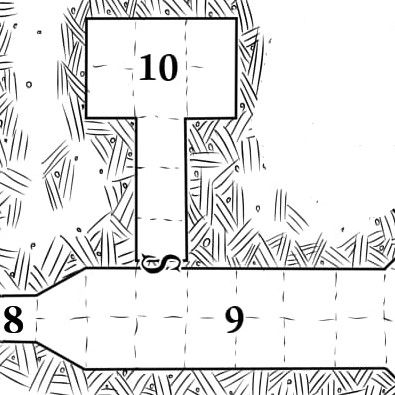
\includegraphics[width=\columnwidth]{pics/map_8-10.jpg}
\subsection{8 : Passage Secret}\label{n2:s8}
\begin{itemize}
  \item Directement sous \textbf{\nameref{n1:s7}}
  \item \'Etroite alcôve s’élargissant sur \textbf{\nameref{n2:s9}}
\end{itemize}

\subsection{9 : Hall aux Statues}\label{n2:s9}
Un long et large couloir. 
\begin{itemize}
  \item Six énormes sculptures d’hommes-serpents en armes et armures
  \item Regard dédaigneux
  \item $1^{ère}$ à gauche : légèrement désalignée
  \item  déplacée, révèle \textbf{\nameref{n2:s10}}
\end{itemize}

\vfill\break
\subsection{10 : Salle de Garde Secrète}\label{n2:s10}
Cette pièce fut autrefois une salle de garde secrète pour
les assassins du temple. 

\begin{itemize}
  \item Aujourd'hui vide et sombre. 
  \item Les meubles ont pourri jusqu’à se désagréger. 
  \item Deux guisarmes sont toujours utilisables
  \item Une icône religieuse en argent valant 50 PO.
\end{itemize}